\documentclass[11pt]{article}

% ---------- Page & fonts ----------
\usepackage[margin=1in]{geometry}
\usepackage[utf8]{inputenc}
\usepackage[T1]{fontenc}

% ---------- Math ----------
\usepackage{amsmath, amssymb, amsthm, mathtools}

% ---------- Graphs / figures ----------
\usepackage{tikz}
\usetikzlibrary{positioning, arrows.meta, calc}

% ---------- Quality of life ----------
\usepackage{enumitem}
\usepackage{hyperref}
\usepackage{cleveref}
\usepackage{xcolor}

\hypersetup{
  colorlinks=true,
  linkcolor=blue!50!black,
  citecolor=blue!50!black,
  urlcolor=blue!50!black
}

% ================= Theorem environments =================
\theoremstyle{plain}
\newtheorem{theorem}{Theorem}[section]
\newtheorem{lemma}[theorem]{Lemma}
\newtheorem{proposition}[theorem]{Proposition}
\newtheorem{corollary}[theorem]{Corollary}
\newtheorem{conjecture}[theorem]{Conjecture}

\theoremstyle{definition}
\newtheorem{definition}[theorem]{Definition}
\newtheorem{example}[theorem]{Example}

\theoremstyle{remark}
\newtheorem{remark}[theorem]{Remark}

% ================= Macros =================
\newcommand{\Nout}{N^{+}}

\tikzset{
    vertex/.style={circle, draw=black, fill=black, inner sep=1.8pt},
    kern/.style={circle, draw=black, fill=white, very thick, inner sep=2.6pt}
}

% ================= Document =================
\title{Hereditary Classes of Digraphs with $2$-d Kernels Are Arcless}
\author{%
  Siddharth Narayan Mishra\\[0.2em]
  \small Roll No.\ 123CS0189\\
  \small Department of Computer Science and Engineering\\
  \small National Institute of Technology Rourkela%
}
\date{\today}

\begin{document}

\maketitle

\begin{abstract}
\noindent
We prove that a class of finite digraphs closed under induced subdigraphs has the property
that every one of its members possesses a $2$-d kernel if and only if every one of its
members has no arcs. Since any class defined by forbidding structures is closed under induced
subdigraphs, it follows that no class containing a digraph with an arc carries $2$-d kernels the way
Richardson's theorem makes ordinary kernels available. The obstruction is a single arc.
\end{abstract}

\section{Definitions}

We fix our conventions completely, so that nothing beyond elementary set theory is assumed.

\begin{definition}[Digraph]
A \emph{digraph} is a pair $D = (V, A)$ in which $V$ is a finite set, whose elements are
called \emph{vertices}, and $A$ is a set of ordered pairs of \emph{distinct} vertices, whose
elements are called \emph{arcs}. We write $uv$ for the arc $(u,v)$ and say that $uv$ goes
\emph{from} $u$ \emph{to} $v$.
\end{definition}

Requiring the two entries of an arc to be distinct simply says that no vertex has an arc to
itself. We allow both $uv \in A$ and $vu \in A$ to hold simultaneously.

\begin{definition}[Out-neighbourhood]
For a vertex $v$ of $D = (V,A)$, the \emph{out-neighbourhood} of $v$ is
\[
  \Nout(v) \;=\; \{\, w \in V \;:\; vw \in A \,\}.
\]
\end{definition}

\begin{definition}[Independent set]
A set $K \subseteq V$ is \emph{independent} in $D = (V,A)$ if for all distinct $u, v \in K$
neither $uv \in A$ nor $vu \in A$. That is, no arc has both of its vertices in $K$.
\end{definition}

\begin{definition}[Induced subdigraph]
For $S \subseteq V$, the \emph{subdigraph of $D$ induced by $S$} is the digraph
\[
  D[S] \;=\; \bigl(\, S,\; \{\, uv \in A \;:\; u \in S \text{ and } v \in S \,\} \,\bigr).
\]
So $D[S]$ keeps the vertices in $S$ and keeps exactly those arcs of $D$ whose two vertices
both lie in $S$.
\end{definition}

\begin{definition}[$2$-d kernel]\label{def:2dk}
Let $D = (V,A)$ be a digraph. A set $K \subseteq V$ is a \emph{$2$-d kernel} of $D$ if
\begin{enumerate}[label=(\roman*)]
  \item\label{it:indep} $K$ is independent in $D$; and
  \item\label{it:dom} every $v \in V \setminus K$ satisfies
        $\lvert \Nout(v) \cap K \rvert \geq 2$.
\end{enumerate}
\end{definition}

Condition \ref{it:dom} says that every vertex outside $K$ has arcs to at least two
\emph{different} vertices of $K$. The letter \emph{d} records that the domination
requirement is a $2$-domination requirement. This is the notion written $2$-kernel in earlier
drafts of this project; the letter is added here to keep it apart from the distance-based
$k$-kernel of the published literature, which is a different notion, requiring the vertices
of $K$ to be pairwise far apart rather than requiring them to be reached twice.

\begin{definition}[Closed under induced subdigraphs]\label{def:hered}
A class $\mathcal{C}$ of digraphs is \emph{closed under induced subdigraphs} if for every
$D \in \mathcal{C}$ and every $S \subseteq V(D)$ we have $D[S] \in \mathcal{C}$.
\end{definition}

\begin{definition}[Arcless]
A digraph $D = (V,A)$ is \emph{arcless} if $A = \varnothing$.
\end{definition}

\section{Two lemmas}

The first lemma is the entire content of the matter. A $2$-d kernel cannot be small.

\begin{lemma}[Size lemma]\label{lem:size}
Let $K$ be a $2$-d kernel of a digraph $D = (V,A)$. If $V \setminus K \neq \varnothing$,
then $\lvert K \rvert \geq 2$.
\end{lemma}

\begin{proof}
Since $V \setminus K$ is non-empty, we may choose a vertex $v \in V \setminus K$. By
condition \ref{it:dom} of Definition~\ref{def:2dk},
\[
  \lvert \Nout(v) \cap K \rvert \;\geq\; 2 .
\]
The set $\Nout(v) \cap K$ is a subset of $K$, so $\lvert K \rvert \geq \lvert \Nout(v) \cap K \rvert$.
Combining the two inequalities gives $\lvert K \rvert \geq 2$.
\end{proof}

\begin{lemma}\label{lem:twovertex}
Let $D = (V,A)$ be a digraph with $\lvert V \rvert = 2$ and $A \neq \varnothing$. Then $D$
has no $2$-d kernel.
\end{lemma}

\begin{proof}
Write $V = \{u, v\}$. Since $A \neq \varnothing$ and every arc joins two distinct vertices of
$V$, after relabelling we may assume $uv \in A$.

Suppose, for contradiction, that $K$ is a $2$-d kernel of $D$. As $K \subseteq V$ there are
exactly two possibilities.

\medskip
\noindent\textbf{Case 1: $K = V$.} Then $u$ and $v$ are distinct elements of $K$ and
$uv \in A$, so $K$ is not independent. This contradicts condition \ref{it:indep} of
Definition~\ref{def:2dk}.

\medskip
\noindent\textbf{Case 2: $K \subsetneq V$.} Then $V \setminus K \neq \varnothing$, so
Lemma~\ref{lem:size} gives $\lvert K \rvert \geq 2$. But $K \subseteq V$ and
$\lvert V \rvert = 2$, so $\lvert K \rvert \leq 2$. Hence $\lvert K \rvert = 2$, and a subset
of a two-element set having two elements is the whole set, so $K = V$. This contradicts
$K \subsetneq V$.

\medskip
Both cases are impossible, so no $2$-d kernel exists.
\end{proof}

Note that Case 2 covers $K = \varnothing$, since the empty set is a proper subset of $V$.
Note also that the lemma covers both two-vertex digraphs that possess an arc: the one with
a single arc, and the one with a pair of opposite arcs.

\begin{example}\label{ex:loss}
A digraph may have a $2$-d kernel while an induced subdigraph of it has none. Let $D$ have
vertices $u, a, b$ and arcs $ua$ and $ub$. Then $K = \{a,b\}$ is a $2$-d kernel of $D$: it is
independent, since $D$ has no arc between $a$ and $b$, and the only vertex outside it is $u$,
which has arcs to both of its elements. Deleting $b$ leaves $D[\{u,a\}]$, which has the
single arc $ua$ and, by Lemma~\ref{lem:twovertex}, no $2$-d kernel at all.
\begin{center}
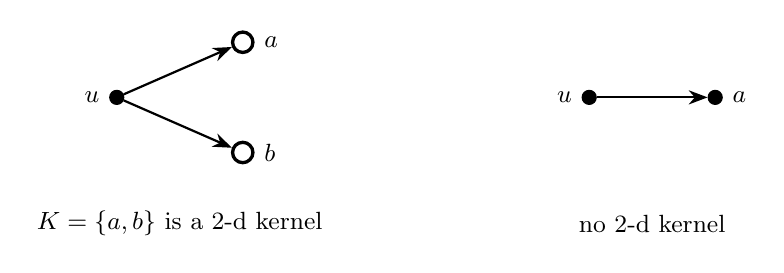
\begin{tikzpicture}[>={Stealth[length=2.4mm]}, every node/.style={font=\small}]
  \node[vertex, label=left:$u$]   (u)  at (0,0)    {};
  \node[kern,   label=right:$a$]  (a)  at (1.6,0.7){};
  \node[kern,   label=right:$b$]  (b)  at (1.6,-0.7){};
  \draw[->, thick] (u) -- (a);
  \draw[->, thick] (u) -- (b);
  \node at (0.8,-1.6) {$K=\{a,b\}$ is a $2$-d kernel};

  \node[vertex, label=left:$u$]  (u2) at (6,0)   {};
  \node[vertex, label=right:$a$] (a2) at (7.6,0) {};
  \draw[->, thick] (u2) -- (a2);
  \node at (6.8,-1.6) {no $2$-d kernel};
\end{tikzpicture}
\end{center}
\end{example}

\section{The theorem}

\begin{theorem}\label{thm:main}
Let $\mathcal{C}$ be a class of finite digraphs that is closed under induced subdigraphs.
Then every member of $\mathcal{C}$ has a $2$-d kernel if and only if every member of
$\mathcal{C}$ is arcless.
\end{theorem}

\begin{proof}
\textbf{($\Leftarrow$)} Suppose every member of $\mathcal{C}$ is arcless, and let
$D = (V,A) \in \mathcal{C}$, so that $A = \varnothing$. Take $K = V$. Condition
\ref{it:indep} holds because $D$ has no arcs at all, so in particular no arc has both
vertices in $K$. Condition \ref{it:dom} holds vacuously, because $V \setminus K = \varnothing$
and so there is no vertex to which the requirement applies. Hence $K$ is a $2$-d kernel of
$D$.

\medskip
\noindent\textbf{($\Rightarrow$)} Suppose every member of $\mathcal{C}$ has a $2$-d kernel,
and suppose for contradiction that some $D = (V,A) \in \mathcal{C}$ is not arcless. Choose an
arc $uv \in A$. By the definition of a digraph, $u \neq v$.

Put $S = \{u, v\}$, so $S \subseteq V$ and $\lvert S \rvert = 2$. Both vertices of the arc
$uv$ lie in $S$, so $uv$ is an arc of $D[S]$, and therefore $D[S]$ has at least one arc.

Since $\mathcal{C}$ is closed under induced subdigraphs and $S \subseteq V(D)$, we have
$D[S] \in \mathcal{C}$. By hypothesis, $D[S]$ has a $2$-d kernel. But $D[S]$ has exactly two
vertices and at least one arc, so by Lemma~\ref{lem:twovertex} it has no $2$-d kernel. This is a
contradiction.

Hence no member of $\mathcal{C}$ has an arc.
\end{proof}

\begin{corollary}\label{cor:vacuous}
Let $D$ be a digraph such that every induced subdigraph of $D$ has a $2$-d kernel. Then $D$
is arcless.
\end{corollary}

\begin{proof}
Let $\mathcal{C} = \{\, D[S] \;:\; S \subseteq V(D) \,\}$ be the class of all induced
subdigraphs of $D$.

First, $\mathcal{C}$ is closed under induced subdigraphs. Indeed, a member of $\mathcal{C}$
is $D[S]$ for some $S \subseteq V(D)$, and a subset of its vertex set is a set $T \subseteq S$.
By Definition~\ref{def:hered} we must check that $(D[S])[T] \in \mathcal{C}$. Now $(D[S])[T]$ has vertex
set $T$, and its arcs are the arcs of $D[S]$ with both vertices in $T$, which are exactly the
arcs of $D$ with both vertices in $T$, since $T \subseteq S$. So $(D[S])[T] = D[T]$, which
lies in $\mathcal{C}$ because $T \subseteq V(D)$.

Second, every member of $\mathcal{C}$ has a $2$-d kernel, by hypothesis.

By Theorem~\ref{thm:main}, every member of $\mathcal{C}$ is arcless. Taking $S = V(D)$ gives
$D = D[V(D)] \in \mathcal{C}$, so $D$ is arcless.
\end{proof}

\section{Why ordinary kernels escape this}

\begin{definition}[Kernel]
A set $K \subseteq V$ is a \emph{kernel} of $D = (V,A)$ if $K$ is independent and every
$v \in V \setminus K$ satisfies $\lvert \Nout(v) \cap K \rvert \geq 1$.
\end{definition}

\begin{remark}\label{rem:contrast}
The proof of Lemma~\ref{lem:size} applied to a kernel yields only $\lvert K \rvert \geq 1$, which
is no restriction. Accordingly Lemma~\ref{lem:twovertex} has no analogue: in the digraph on
$\{u,v\}$ with the single arc $uv$, the set $K = \{v\}$ \emph{is} a kernel, since it is
independent and $u$ has an arc into it.

This is the whole of the difference. A kernel may consist of one vertex; a $2$-d kernel may
not, as soon as any vertex lies outside it, because two arcs from one vertex must have two
distinct heads. Heredity forces us down to induced subdigraphs on two vertices, and at that
size a $2$-d kernel has no room to exist unless there are no arcs.

For kernels the corresponding programme therefore succeeds. Richardson's theorem states that
every digraph with no directed cycle of odd length has a kernel. The class of such digraphs
is closed under induced subdigraphs, because deleting vertices cannot create a directed cycle
that was not already present. Hence for such a digraph every induced subdigraph again has no
odd directed cycle and so again has a kernel.
\end{remark}

\begin{remark}\label{rem:noforbidden}
Theorem~\ref{thm:main} rules out every attempt to recover heredity by forbidding structures.
Let $\mathcal{F}$ be any family of digraphs and let $\operatorname{Forb}(\mathcal{F})$ be the
class of digraphs having no induced subdigraph isomorphic to a member of $\mathcal{F}$. This
class is closed under induced subdigraphs, because an induced subdigraph of an induced
subdigraph of $D$ is again an induced subdigraph of $D$, as computed in the proof of
Corollary~\ref{cor:vacuous}. Theorem~\ref{thm:main} therefore applies to it: every member of
$\operatorname{Forb}(\mathcal{F})$ has a $2$-d kernel if and only if every member is arcless.
Hence no choice of $\mathcal{F}$ produces a class that contains a digraph with an arc and on
which $2$-d kernels are guaranteed.

In particular, no condition on directed cycles can help. Let $A_1$ be the digraph on two
vertices $u, v$ with the single arc $uv$. It contains no directed cycle of any length, so it
lies in every class defined by forbidding directed cycles, and in particular in the class of
digraphs with no odd directed cycle to which Richardson's theorem applies. By
Lemma~\ref{lem:twovertex}, $A_1$ has no $2$-d kernel.
\end{remark}

\section{Consequence for the kernel method}

The kernel lemma of Bondy, Boppana and Siegel, which appears as Lemma 1 of Chapter 33 of
Aigner and Ziegler's \emph{Proofs from THE BOOK}, states that if every induced subdigraph of
an orientation $\vec{G}$ of $G$ has a kernel, and $\lvert C(v) \rvert \geq d^{+}(v) + 1$ for
every vertex $v$, then there is a colouring $c$ of $V$ with $c(v) \in C(v)$ for every $v$ and
$c(u) \neq c(v)$ for every edge $uv$ of $G$. The hypothesis is required of every induced
subdigraph, and not of $\vec{G}$ alone, because the proof applies it to the set
$A(c) = \{\, v \in V : c \in C(v) \,\}$ for a colour $c$; the lists are arbitrary, so $A(c)$
may be any subset of $V$.

Now consider any statement obtained from that lemma by replacing the word \emph{kernel} by
\emph{$2$-d kernel} in its hypothesis, whatever conclusion that statement may assert. By
Corollary~\ref{cor:vacuous} its hypothesis holds only when $\vec{G}$ is arcless. In that case
$G$ has no edges, and the condition $\lvert C(v) \rvert \geq d^{+}(v) + 1 = 1$ makes every
list non-empty, so choosing any $c(v) \in C(v)$ already gives a colouring of the required
kind. Such a statement therefore asserts nothing that is not immediate, whatever bound it
claims.

\begin{remark}
The motivation for wanting such a replacement is that a $2$-d kernel deletes two
out-neighbours of an uncoloured vertex in exchange for the single colour that vertex loses,
rather than one, which suggests a bound in the region of $\lceil d^{+}(v)/2 \rceil + 1$ in
place of $d^{+}(v) + 1$. No such bound is proved here, and none is needed: the argument above
rejects the hereditary hypothesis whatever conclusion is drawn from it.

This closes the hereditary form of the method and nothing else. It says nothing about which
individual digraphs possess $2$-d kernels, and it does not by itself close variants in which
the hypothesis is required not of every induced subdigraph but only of the colour classes
that the induction actually processes.
\end{remark}

\end{document}
